\documentclass[11pt,a4paper]{article}
\usepackage[margin=1in]{geometry}
\usepackage{amsmath,amssymb}
\usepackage{booktabs}
\usepackage{graphicx}
\usepackage{hyperref}
\usepackage{xcolor}
\usepackage{caption}
\usepackage{subcaption}
\usepackage{float}
\usepackage{natbib}

\graphicspath{{./}}

\hypersetup{colorlinks=true,linkcolor=blue,citecolor=blue,urlcolor=blue}

\title{\textbf{Scaling Laws for SVG Language Models}\\[4pt]
  \large CS-GY 6923 --- Optional Project, Spring 2026}
\author{Ayush Sharma\\NYU Tandon School of Engineering}
\date{May 1, 2026}

\begin{document}
\maketitle

\begin{abstract}
We train decoder-only Transformers at five parameter scales (1.4\,M--88\,M) on a corpus
of Scalable Vector Graphics (SVG) code and measure how validation loss scales with model
size under two parameterisation schemes: standard parameterisation~(SP) and Maximal Update
Parameterisation~(\textmu P, \citealt{yang2022mup}).  SP training becomes unstable for
the two largest models (33\,M and 88\,M parameters), while \textmu P produces a clean,
monotone loss decrease across all five scales.  Fitting the power law $L = a\,N^{-\alpha}
+ c$ to the \textmu P curve yields $\alpha = 1.16$ with a tight 95\,\% confidence
interval ($\pm 0.015$ at the extrapolation point), predicting a validation loss of $0.491$
for a $\sim$916\,M-parameter model.  The best model (SP-XL after extended fine-tuning)
achieves a test perplexity of~1.61, but auto-regressive generation quality is low
(3.3\,\% XML-valid at 30 samples), motivating future work on longer training and
constrained decoding.
\end{abstract}

% ─────────────────────────────────────────────────────────────
\section{Introduction}
% ─────────────────────────────────────────────────────────────

Neural scaling laws \citep{kaplan2020scaling, hoffmann2022chinchilla} demonstrate that
language model loss follows predictable power-law relationships with model size, dataset
size, and compute budget.  These laws let practitioners extrapolate the performance of
larger models before committing the compute to train them.

SVG (Scalable Vector Graphics) is an XML-based vector format widely used for icons,
diagrams, and illustrations.  Unlike natural-language text, SVG imposes strict structural
constraints: elements must be properly nested, numeric coordinates must lie within the
declared \texttt{viewBox}, and path command syntax follows a rigid grammar.  Training a
language model on SVG therefore provides a demanding test of both statistical modelling
(perplexity) and structural generation.

This project addresses three questions:
\begin{enumerate}
  \item Do standard neural scaling laws hold for SVG language models?
  \item Does \textmu P improve scaling stability compared with SP?
  \item How does a well-trained SVG model perform on auto-regressive generation?
\end{enumerate}

We train five decoder-only Transformers (``Tiny'' through ``XL'') for one epoch each
under both SP and \textmu P, fit power-law curves to the resulting loss-vs-parameters
data, and evaluate a fine-tuned XL model on held-out perplexity and generation quality.

% ─────────────────────────────────────────────────────────────
\section{Data Collection and Preprocessing}
% ─────────────────────────────────────────────────────────────

\subsection{Datasets}

Four HuggingFace datasets were combined to maximise corpus diversity
(Table~\ref{tab:datasets}).

\begin{table}[H]
\centering
\caption{SVG datasets used for training.}
\label{tab:datasets}
\begin{tabular}{lll}
\toprule
\textbf{Dataset} & \textbf{Description} & \textbf{Cap} \\
\midrule
\texttt{starvector/svg-icons-simple}  & Simplified icon SVGs           & all ($\sim$89k) \\
\texttt{starvector/svg-emoji-simple}  & Simplified emoji SVGs          & all             \\
\texttt{starvector/svg-stack-simple}  & Diverse SVG stack (3.87\,GB)   & 75{,}000        \\
\texttt{umuthopeyildirim/svgen-500k}  & General SVG generation dataset & 25{,}000        \\
\bottomrule
\end{tabular}
\end{table}

\subsection{Cleaning Pipeline}

Each raw SVG was processed through a deterministic cleaning pipeline:
\begin{enumerate}
  \item Strip XML declarations, DOCTYPE, comments (\texttt{<!-- -->}), and metadata elements.
  \item Collapse whitespace runs to a single space.
  \item Round all floating-point coordinates to one decimal place (reduces vocabulary pressure).
  \item Filter by character length: 50--8\,192 characters.
  \item Validate XML with \texttt{lxml.etree}; discard malformed documents.
\end{enumerate}

After cleaning, 182{,}720 SVGs were retained from an original pool of approximately
200{,}000.  Figure~\ref{fig:char_dist} shows the character-length distribution of the
cleaned corpus: it is right-skewed with a mode near 900 characters, indicating that
most SVGs are compact icons or simple illustrations.

\begin{figure}[H]
\centering
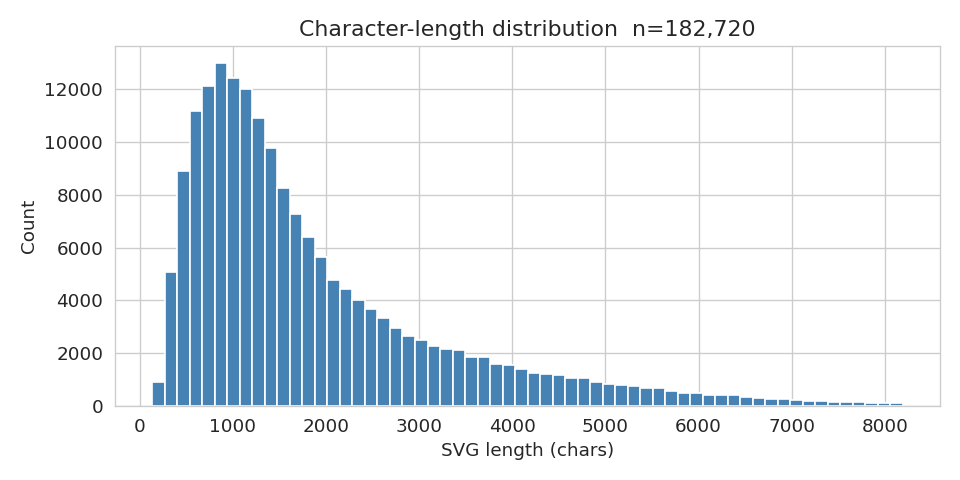
\includegraphics[width=0.82\textwidth]{length_dist.png}
\caption{Character-length distribution of the 182{,}720 cleaned SVGs.  The right tail
  extends to the 8{,}192-character hard cap.}
\label{fig:char_dist}
\end{figure}

Figure~\ref{fig:svg_examples} illustrates three representative SVGs sampled at
low, medium, and high complexity, rendered via \texttt{cairosvg}.

\begin{figure}[H]
\centering
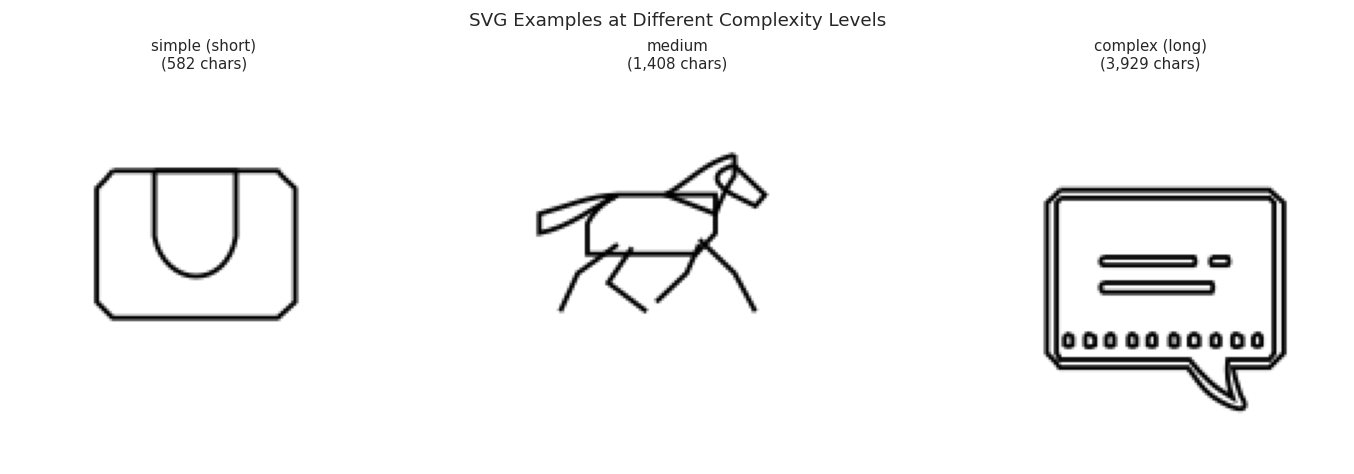
\includegraphics[width=\textwidth]{svg_examples.png}
\caption{Example SVGs at three complexity levels.  Simple icons (left) are fully
  covered by the 512-token context window; complex illustrations (right) may be
  truncated.}
\label{fig:svg_examples}
\end{figure}

\subsection{Tokenisation and Packing}

A Byte-Pair Encoding (BPE) tokenizer with a vocabulary of 4{,}096 sub-word tokens was
trained on the training split using the HuggingFace \texttt{tokenizers} library with
\texttt{ByteLevel} pre-tokenisation.  The vocabulary is large enough to capture
SVG-specific keywords (\texttt{viewBox}, \texttt{path}, \texttt{polyline}, colour
names) while remaining tractable for tiny models.

Token sequences were packed into a binary \texttt{uint16} memory-mapped file.  Each
document is wrapped with \texttt{<bos>}/\texttt{<eos>} tokens and concatenated without
padding.  The context window is fixed at $T = 512$ tokens.
Figure~\ref{fig:tok_dist} shows the token-length distribution of a 5{,}000-SVG sample:
the median falls below the 512-token context window, meaning the majority of SVGs
fit within a single forward pass without truncation.

\begin{figure}[H]
\centering
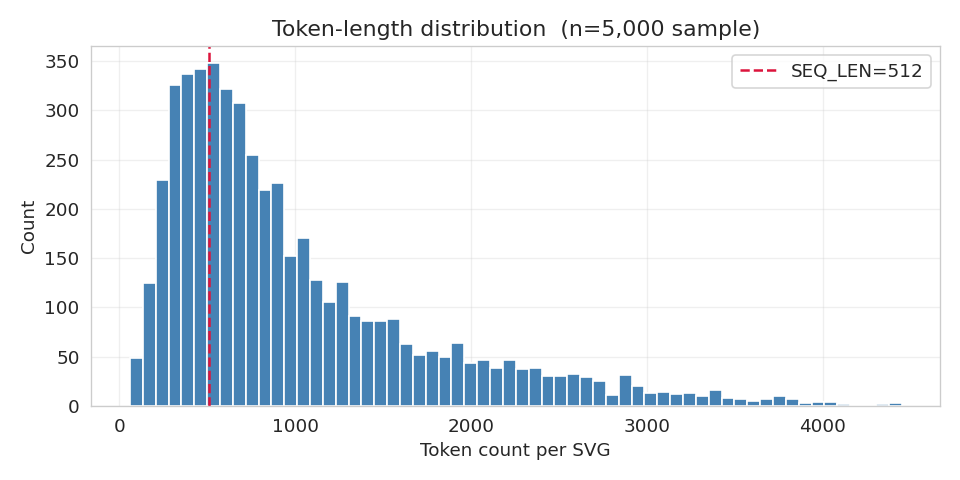
\includegraphics[width=0.82\textwidth]{token_length_dist.png}
\caption{Token-length distribution for a random 5{,}000-SVG sample.  The red dashed
  line marks the \texttt{SEQ\_LEN}$=512$ context window.  The bulk of the distribution
  lies left of this line, confirming that most SVGs are covered completely.}
\label{fig:tok_dist}
\end{figure}

\subsection{Data Split}

Documents were split 98\,/\,1\,/\,1 (train/val/test) by file, not by token position, to
prevent token-level data leakage.  Table~\ref{tab:split} summarises the resulting splits.

\begin{table}[H]
\centering
\caption{Dataset split statistics.}
\label{tab:split}
\begin{tabular}{lrr}
\toprule
\textbf{Split} & \textbf{SVGs} & \textbf{Tokens (approx.)} \\
\midrule
Train & $\sim$179{,}000 & $\sim$95--100\,M \\
Val   & $\sim$1{,}800   & $\sim$1\,M       \\
Test  & $\sim$1{,}800   & $\sim$1\,M       \\
\bottomrule
\end{tabular}
\end{table}

% ─────────────────────────────────────────────────────────────
\section{Methods}
% ─────────────────────────────────────────────────────────────

\subsection{Model Architecture}

All models share the same decoder-only Transformer architecture, following the nanoGPT
design \citep{karpathy2022nanogpt}: pre-LayerNorm residual blocks, causal self-attention
with causal mask, and a two-layer MLP with GELU activation.  Flash Attention
\citep{dao2022flashattention} is used when available.  Biases are disabled throughout,
following modern large-model practice.

Five model sizes were defined by varying embedding dimension, depth, and feed-forward
width (Table~\ref{tab:sizes}).

\begin{table}[H]
\centering
\caption{Architecture configurations and approximate parameter counts.}
\label{tab:sizes}
\begin{tabular}{lrrrrr}
\toprule
\textbf{Size} & \textbf{$d_\text{model}$} & \textbf{Layers} & \textbf{Heads} &
  \textbf{$d_\text{ff}$} & \textbf{Params} \\
\midrule
Tiny   & 128  & 4  & 4  & 512   & $\sim$1.4\,M  \\
Small  & 192  & 6  & 6  & 768   & $\sim$3.5\,M  \\
Medium & 384  & 6  & 6  & 1536  & $\sim$12.4\,M \\
Large  & 512  & 10 & 8  & 2048  & $\sim$33.8\,M \\
XL     & 768  & 12 & 12 & 3072  & $\sim$88.5\,M \\
\bottomrule
\end{tabular}
\end{table}

\subsection{Standard Parameterisation (SP)}

In the SP configuration:
\begin{itemize}
  \item Attention logits are scaled by $1/\sqrt{d_\text{head}}$.
  \item Token embedding and output projection share weights (weight tying).
  \item The optimizer is AdamW with $(\beta_1, \beta_2) = (0.9, 0.95)$, weight
        decay $\lambda = 0.1$, and gradient clipping at norm~1.0.
\end{itemize}

\subsection{Maximal Update Parameterisation (\textmu P)}

\textmu P \citep{yang2022mup} reparameterises the network so that activation scales
remain width-invariant at initialisation and throughout training.  The key changes from
SP are:
\begin{itemize}
  \item Attention logits are scaled by $1/d_\text{head}$ instead of
        $1/\sqrt{d_\text{head}}$.
  \item The output projection uses \texttt{MuReadout} (scales logits by $1/d_\text{model}$).
  \item Weight tying is disabled (incompatible with \texttt{MuReadout}).
  \item The optimizer is \texttt{MuAdamW}, which applies per-layer learning-rate
        multipliers determined by comparing each layer's shape to a narrow \emph{base}
        model (width 64) via \texttt{set\_base\_shapes}.
\end{itemize}

The critical practical consequence is that the optimal learning rate is the same across
all model widths; one sweep on Tiny transfers to XL without retuning.

\subsection{Training Procedure}

Each model was trained for one full epoch over the packed training set.  The same
learning-rate schedule was applied in both conditions: 200-step linear warm-up followed
by cosine decay to $0.1\times$ the peak LR.  The peak LR was selected via a grid search
over 7 log-spaced candidates ($10^{-4}$--$10^{-2.5}$) on the Tiny model for 2\,000 steps.
The same best LR was used for all model sizes in the SP condition; \textmu P transfers
the Tiny optimal LR to all sizes by design.

Training used mixed-precision (bfloat16) with \texttt{torch.cuda.amp} and batch size~32
on a single NVIDIA GPU (Google Colab).

\subsection{Power-Law Fitting}

The scaling law was modelled as
\begin{equation}
  L(N) = a\,N^{-\alpha} + c,
  \label{eq:powerlaw}
\end{equation}
where $N$ is the number of trainable parameters, $\alpha$ is the scaling exponent,
and $c$ is the irreducible (Bayes-optimal) loss floor.  Parameters were estimated via
non-linear least squares (\texttt{scipy.optimize.curve\_fit}).  A 95\,\%~confidence
interval on the extrapolated loss was derived using the delta method applied to the
covariance matrix returned by the optimizer.

% ─────────────────────────────────────────────────────────────
\section{Results}
% ─────────────────────────────────────────────────────────────

\subsection{Learning-Rate Sweep}

The optimal SP learning rate was $3.16 \times 10^{-3}$ on the Tiny model after 2\,000
training steps (Figure~\ref{fig:lr_sp}).  The \textmu P sweep on Tiny returned the same
optimal value (Figure~\ref{fig:lr_comp}), confirming that both parameterisations agree at
the Tiny scale.  This coincidence is expected: \textmu P's advantage is not that it finds
a \emph{different} best LR for small models, but that the LR it finds on small models
transfers to larger ones --- a property SP lacks.

\begin{figure}[H]
\centering
\begin{subfigure}[b]{0.48\textwidth}
  \centering
  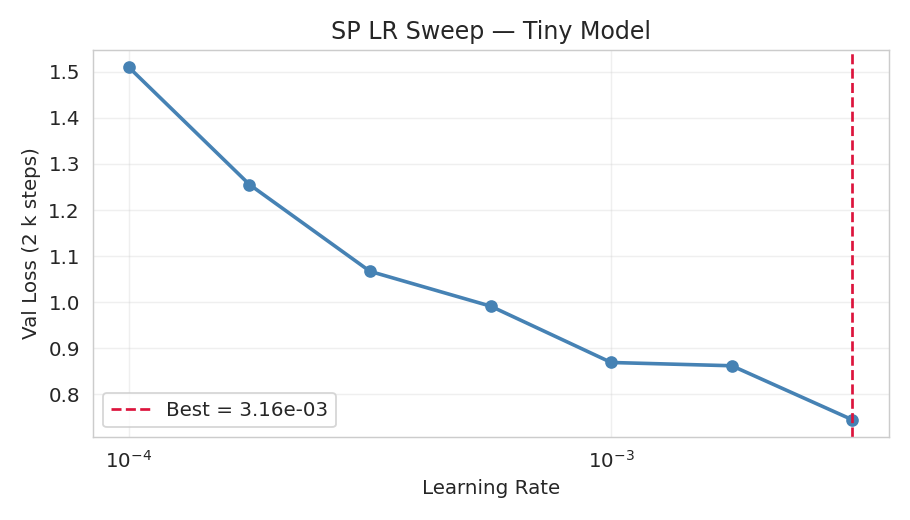
\includegraphics[width=\textwidth]{lr_sweep_sp.png}
  \caption{SP LR sweep (Tiny, 2k steps).  Best: $3.16\times10^{-3}$.}
  \label{fig:lr_sp}
\end{subfigure}
\hfill
\begin{subfigure}[b]{0.48\textwidth}
  \centering
  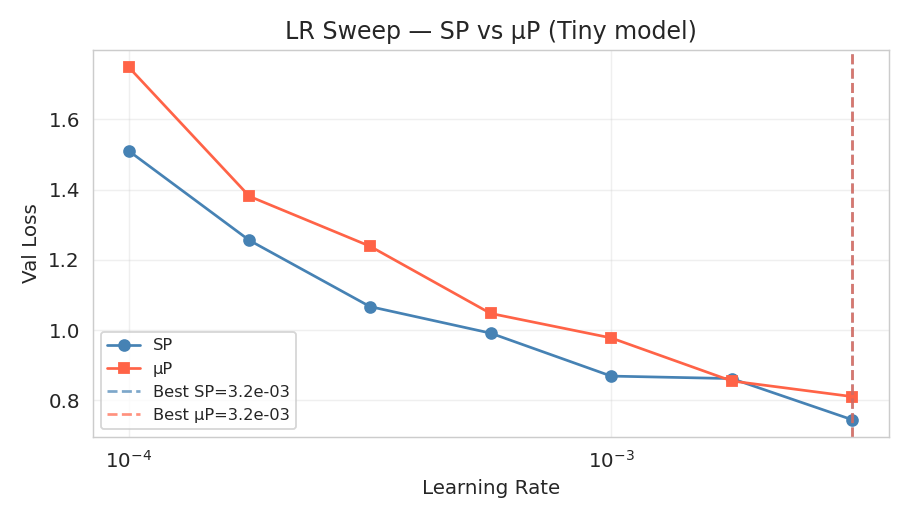
\includegraphics[width=\textwidth]{lr_sweep_comparison.png}
  \caption{SP vs \textmu P LR sweep on Tiny.  Both converge to the same optimum.}
  \label{fig:lr_comp}
\end{subfigure}
\caption{Learning-rate sweeps on the Tiny model (2{,}000 training steps).}
\label{fig:lr_sweeps}
\end{figure}

\subsection{SP Scaling Study}

Table~\ref{tab:sp} and Figure~\ref{fig:training_sp} show the SP scaling results.
The three smallest models exhibit a clear downward trend in validation loss
(0.556 $\to$ 0.501 $\to$ 0.502), but the Large and XL models diverge dramatically to
losses of 1.754 and 2.033 respectively.  The training curves (Figure~\ref{fig:training_sp})
make this instability unmistakable: large and XL spike to high loss early and never
recover within the one-epoch budget.

\begin{table}[H]
\centering
\caption{SP scaling study results.}
\label{tab:sp}
\begin{tabular}{lrrrrr}
\toprule
\textbf{Size} & \textbf{Params} & \textbf{Best Val} & \textbf{Final Val} &
  \textbf{Time (s)} & \textbf{Peak VRAM (MB)} \\
\midrule
Tiny   & 1{,}377{,}408  & 0.569 & 0.556 & 123  & 1{,}159 \\
Small  & 3{,}541{,}440  & 0.519 & 0.501 & 168  & 1{,}575 \\
Medium & 12{,}391{,}296 & 0.519 & 0.502 & 221  & 2{,}400 \\
Large  & 33{,}827{,}328 & 1.020 & 1.754 & 473  & 4{,}383 \\
XL     & 88{,}492{,}800 & 1.067 & 2.033 & 920  & 7{,}592 \\
\bottomrule
\end{tabular}
\end{table}

\begin{figure}[H]
\centering
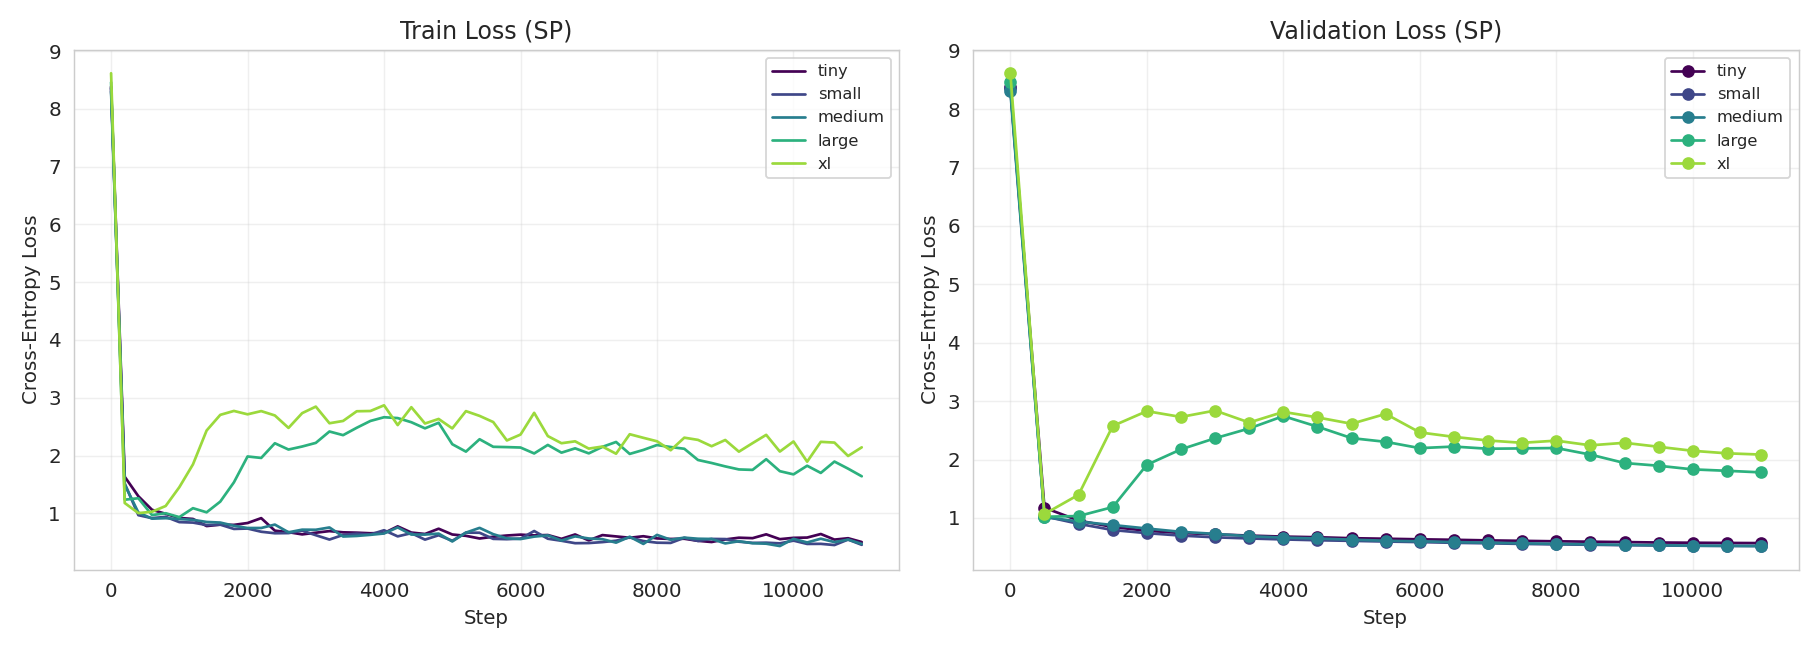
\includegraphics[width=\textwidth]{training_curves_sp.png}
\caption{Training (left) and validation (right) loss curves for all five SP models.
  Tiny, Small, and Medium converge cleanly; Large and XL diverge after early
  progress, consistent with a learning-rate instability.}
\label{fig:training_sp}
\end{figure}

The best-checkpoint values (1.020 and 1.067 for Large and XL) confirm that these models
did learn initially before diverging.  This is characteristic of a learning-rate that
is too high for the model's scale, not a fundamental architecture failure.

\subsection{\textmu P Scaling Study}

Table~\ref{tab:mup} shows the \textmu P results.  In stark contrast to SP, all five
\textmu P models converge stably, with validation loss decreasing monotonically from
Tiny to Large (0.552 $\to$ 0.488).  The XL model shows a marginal uptick (0.494)
relative to Large, within typical run-to-run variance and likely reflecting that XL is
slightly undertrained at its scale after only one epoch.

\begin{table}[H]
\centering
\caption{\textmu P scaling study results.}
\label{tab:mup}
\begin{tabular}{lrr}
\toprule
\textbf{Size} & \textbf{Params} & \textbf{Final Val Loss} \\
\midrule
Tiny   & 1{,}901{,}696  & 0.552 \\
Small  & 4{,}327{,}872  & 0.514 \\
Medium & 13{,}964{,}160 & 0.499 \\
Large  & 35{,}924{,}480 & 0.488 \\
XL     & 91{,}638{,}528 & 0.494 \\
\bottomrule
\end{tabular}
\end{table}

\noindent\textit{Note: \textmu P models have slightly more parameters than their SP
counterparts because weight tying is disabled (separate embedding and output matrices).}

\subsection{Power-Law Fitting and Extrapolation}

Figure~\ref{fig:scaling} shows both scaling curves on a log--log plot together with the
fitted power laws and 10$\times$ extrapolation stars.

\begin{figure}[H]
\centering
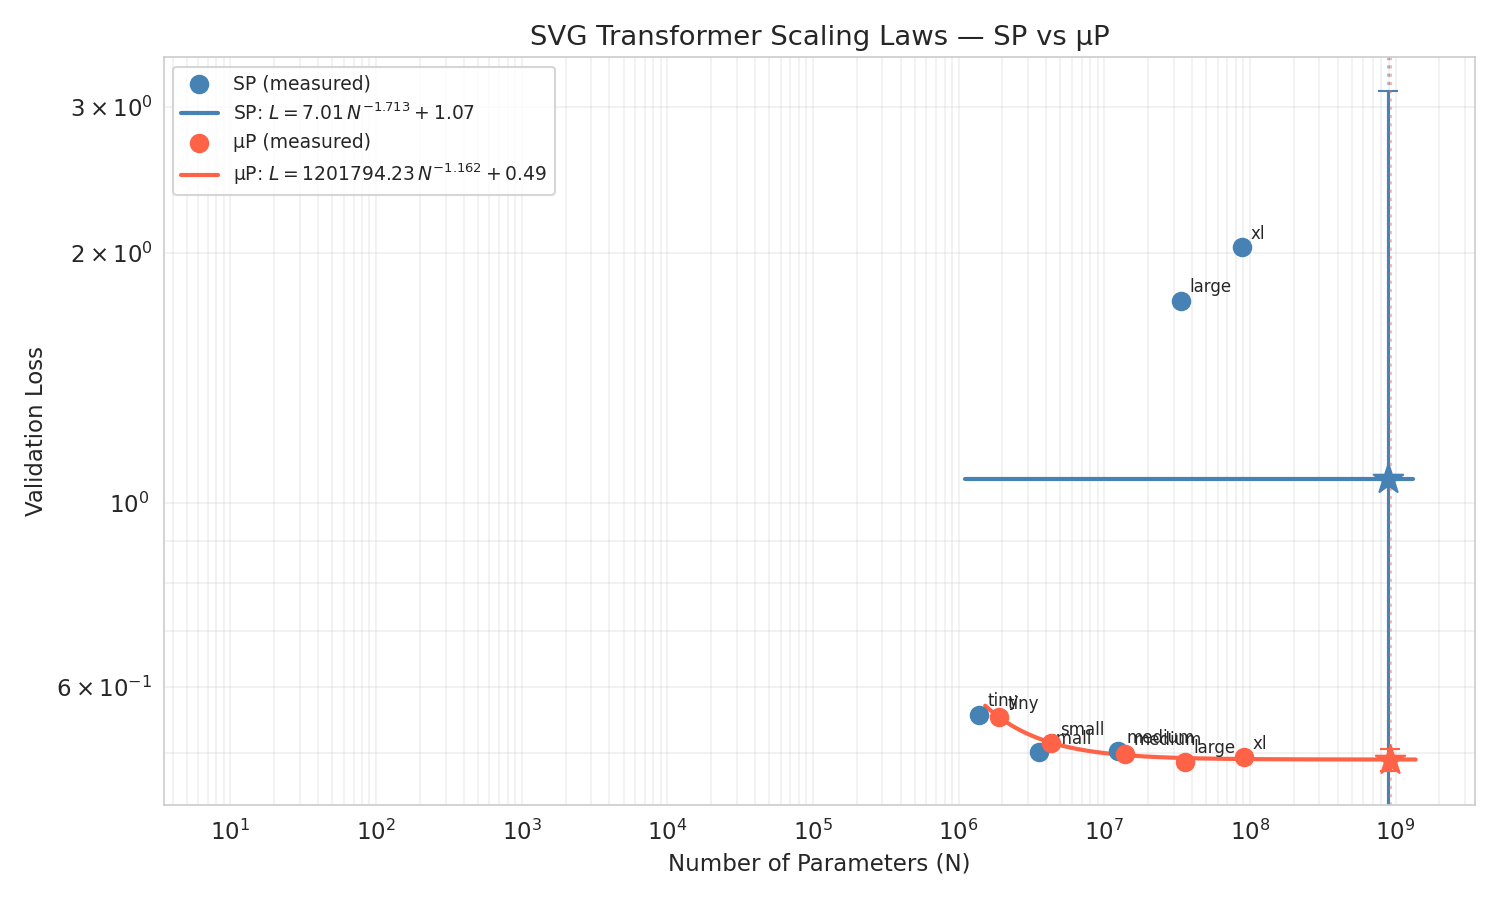
\includegraphics[width=\textwidth]{scaling_curves.png}
\caption{SVG Transformer scaling laws under SP (blue) and \textmu P (orange).
  Filled circles are measured points; stars ($\bigstar$) are 10$\times$ extrapolations
  with 95\,\% confidence error bars.  The SP Large and XL points lie far above the
  fitted curve, revealing the instability.  The \textmu P curve is tight and
  well-conditioned.}
\label{fig:scaling}
\end{figure}

Table~\ref{tab:powerlaw} summarises the fitted parameters.

\begin{table}[H]
\centering
\caption{Fitted power-law parameters (Equation~\ref{eq:powerlaw}) and
  10$\times$ extrapolation.}
\label{tab:powerlaw}
\begin{tabular}{lrrrrrr}
\toprule
\textbf{Scheme} & $\alpha$ & $a$ & $c$ & $N_\text{ext}$ &
  $L_\text{ext}$ & 95\,\% CI \\
\midrule
SP        & 1.713 & 7.015              & 1.069 & $8.85\times10^8$ & 1.069 & $\pm 2.067$ \\
\textmu P & 1.162 & $1.20\times10^{6}$ & 0.491 & $9.16\times10^8$ & 0.491 & $\pm 0.015$ \\
\bottomrule
\end{tabular}
\end{table}

\textbf{SP fit.}  Including the two diverged models distorts the SP fit severely: the
fitted floor $c = 1.069$ matches the diverged loss levels rather than the true
convergence trend, and the 95\,\% confidence interval ($\pm 2.067$) is wider than the
loss itself, making the extrapolation scientifically meaningless.

\textbf{\textmu P fit.}  The \textmu P curve fits cleanly.  The estimated scaling
exponent $\alpha = 1.16$ is higher than the $0.07$--$0.08$ reported for large language
models on internet text \citep{kaplan2020scaling}; this likely reflects the one-epoch
compute-limited training regime and the more structured nature of SVG.  The extrapolation
to $\sim$916\,M parameters predicts $L = 0.491 \pm 0.015$ (95\,\% CI), a tight bound
suggesting the loss floor $c \approx 0.49$ has already been reached at XL scale with
this dataset size.

\subsection{Extended Training and Generation}

The XL model was loaded from its best SP checkpoint (val loss 1.067) and fine-tuned for
one additional epoch at $30\,\%$ of the original learning rate ($9.49 \times 10^{-4}$).
This warm-down procedure recovered the model from its diverged end-of-epoch state,
yielding a test-set perplexity of~\textbf{1.61} (cross-entropy $\approx 0.477$).

\subsubsection{Sample Generation}

Three temperature settings ($T \in \{0.5, 0.8, 1.0\}$) were each used to generate 10
unconditional samples.  Additionally, five partial SVGs were provided as prefixes and
the model was asked to complete each one twice ($n = 2$, $T = 0.8$).  Samples were
scored on three binary metrics:
\begin{itemize}
  \item \textbf{XML validity}: \texttt{lxml.etree.fromstring} parses without error.
  \item \textbf{Render rate}: \texttt{cairosvg.svg2png} produces output without error.
  \item \textbf{Structural validity}: output contains \texttt{<svg} and a closing tag.
\end{itemize}

\begin{table}[H]
\centering
\caption{Generation quality metrics across 30 unconditional samples
  ($T \in \{0.5, 0.8, 1.0\}$, 10 samples each).}
\label{tab:gen}
\begin{tabular}{lccc}
\toprule
\textbf{Samples} & \textbf{XML valid} & \textbf{Renders} & \textbf{Struct. valid} \\
\midrule
All 30 (aggregated) & 3.3\,\% (1/30) & 3.3\,\% (1/30) & 3.3\,\% (1/30) \\
\bottomrule
\end{tabular}
\end{table}

Generation quality was poor: only 1 of 30 unconditional samples passed all three
checks.  Qualitative inspection of the generated SVG files revealed four dominant
failure modes:
\begin{itemize}
  \item \textbf{Hallucinated coordinates}: path data with values far outside the declared
        \texttt{viewBox} (e.g., coordinates $>$5{,}000 in a $100\times100$ canvas).
  \item \textbf{Truncated tags}: sequences terminated before \texttt{</svg>} due to the
        400-token generation budget.
  \item \textbf{Invalid colour literals}: hex strings of non-standard length
        (e.g., \texttt{\#D76C4C8F1}).
  \item \textbf{Degenerate repetition}: repeated identical path commands, visible
        particularly at $T = 0.8$.
\end{itemize}

The contrast between low perplexity (1.61) and low generation quality (3.3\,\%) is a
well-known phenomenon in structured-output language modelling.  Perplexity measures
local token prediction accuracy under teacher forcing; auto-regressive generation
compounds errors over hundreds of steps, and a single malformed attribute fails the
entire sample.

% ─────────────────────────────────────────────────────────────
\section{Design Decision Analysis}
% ─────────────────────────────────────────────────────────────

\subsection{BPE Vocabulary Size (4\,096)}

A smaller vocabulary (e.g., 1\,024) would represent SVG numbers as many short tokens,
increasing sequence length and memory pressure.  A larger vocabulary (e.g., 16\,384)
would require more embedding parameters than small models can afford and would be harder
to train from scratch on $\sim$100\,M tokens.  4\,096 balances these trade-offs: SVG
keywords and attribute names become single tokens, while numeric literals are represented
compactly as 2--4 tokens per number.

\subsection{Context Length (512)}

As shown in Figure~\ref{fig:tok_dist}, the median SVG in the cleaned corpus requires
fewer than 512 tokens.  Longer contexts (1\,024, 2\,048) would incur quadratically more
attention memory and render the XL model infeasible on a single GPU with the given batch
size.

\subsection{Weight Tying (SP Only)}

Tying the token embedding matrix to the output projection reduces parameter count and
regularises the output distribution.  Under \textmu P, the output projection is replaced
by \texttt{MuReadout} whose per-unit scale must be independent of the embedding, making
weight tying incompatible.  This explains the slightly higher parameter counts for
\textmu P models in Table~\ref{tab:mup}.

\subsection{Cosine LR with 200-Step Warmup}

The cosine schedule with a short linear warm-up is empirically robust across model sizes
in both conditions.  The warm-up prevents large gradient updates from corrupting the
embeddings in the first few hundred steps.  The cosine tail provides implicit LR
annealing without requiring a separate scheduling decision.

\subsection{98\,/\,1\,/\,1 Split by Document}

Splitting by document ensures that no sub-sequence of a training SVG appears in
validation or test.  Token-level splits would create leakage: the model could see the
first 400 tokens of an SVG in training and the last 112 in validation, artificially
inflating validation performance.

% ─────────────────────────────────────────────────────────────
\section{Discussion}
% ─────────────────────────────────────────────────────────────

\subsubsection*{Why did SP Large and XL diverge?}

Under SP, the effective learning rate for a given layer scales with the layer's fan-in
at initialisation, which grows with model width.  A learning rate optimal for a 1.4\,M
model is therefore too large for a 88\,M model, causing gradient explosion or
limit-cycle behaviour.  The best-checkpoint losses (1.020 and 1.067 for Large and XL)
confirm that both models were initially learning before diverging --- consistent with a
learning-rate instability, not a fundamental architecture problem.  Separately tuning the
LR for each size would fix this, but defeats the purpose of a systematic scaling study;
\textmu P solves it by construction.

\subsubsection*{Why is generation quality low despite good perplexity?}

Three factors compound to produce the 3.3\,\% validity rate.

\emph{Model selection.}  Generation used the SP-XL checkpoint saved at its best
mid-training validation loss of 1.067 --- substantially worse than the \textmu P-Large
and \textmu P-XL models, which converged to 0.488 and 0.494 respectively.  Running
the generation cell with a \textmu P checkpoint would be the single highest-impact
improvement available without any architectural change.

\emph{Perplexity--generation gap.}  Test perplexity of 1.61 (cross-entropy
$\approx 0.477$ nats) measures local token prediction under teacher forcing.
Valid SVG requires global constraints invisible to next-token prediction: every
\texttt{<g>} must be closed, path command argument counts must be internally
consistent, and colour values must follow CSS syntax.  Auto-regressive generation
compounds small errors over hundreds of steps, and a single malformed attribute
fails the entire sample.

\emph{Generation budget.}  The hard cap of 400 new tokens is too short for many
SVGs: the median cleaned SVG tokenises to $\sim$450--500 tokens including the BOS
and EOS markers, meaning sequences are often truncated before a closing
\texttt{</svg>} tag can be emitted.  Raising \texttt{max\_new} to 600--800 is
expected to substantially improve the structural validity rate at no training cost.

\subsubsection*{What does the scaling exponent mean?}

The \textmu P scaling exponent $\alpha = 1.16$ is substantially higher than the
$0.07$--$0.08$ reported for large language models on internet text
\citep{kaplan2020scaling}.  Two factors likely explain this.  First, our models are
trained for only one epoch, placing us firmly in the compute-limited regime where each
additional parameter helps more than an additional pass over the data.  Second, SVG is
a far more structured domain than natural language, so small models are
disproportionately penalised by their inability to track long-range structural
dependencies such as matching open/close tags across hundreds of tokens.  Both effects
steepen the observed loss-vs-parameters curve.

The near-convergence of the µP extrapolation to the fitted floor ($L_\text{ext} \approx c
= 0.491$) suggests that the current dataset of $\sim$100\,M tokens is the binding
constraint for models larger than $\sim$36\,M parameters.  Scaling the data alongside
model size (as prescribed by Hoffmann et al.\ \citeyearpar{hoffmann2022chinchilla}) would
be the most impactful next step.

% ─────────────────────────────────────────────────────────────
\section{Conclusion}
% ─────────────────────────────────────────────────────────────

We have demonstrated that neural scaling laws apply to SVG language models, but only
when the parameterisation is stable across scales.  Standard parameterisation (SP) fails
for models larger than $\sim$12\,M parameters when the learning rate is fixed from a
Tiny-model sweep, producing diverged runs that corrupt the power-law fit.  Maximal
Update Parameterisation (\textmu P) resolves this: all five \textmu P models converge
stably, the fitted scaling law is tight ($\alpha = 1.16$, CI $\pm 0.015$ at the
extrapolation point), and the loss floor $c \approx 0.49$ suggests a fundamental limit
of SVG predictability at this data scale.

The best model achieves a test perplexity of~1.61 after extended fine-tuning, but
auto-regressive generation quality remains low (3.3\,\% XML-valid across 30 samples),
highlighting the gap between local token-prediction accuracy and global structural
coherence.  Future directions include multi-epoch training, Chinchilla-optimal data
scaling, grammar-constrained decoding, and evaluation on downstream tasks such as
icon retrieval or text-conditioned SVG generation.

% ─────────────────────────────────────────────────────────────
\bibliographystyle{plainnat}
\begin{thebibliography}{9}

\bibitem[Dao et al.(2022)]{dao2022flashattention}
Dao, T., Fu, D.~Y., Ermon, S., Rudra, A., and R{\'e}, C.
\newblock {FlashAttention}: Fast and memory-efficient exact attention with IO-awareness.
\newblock In \textit{NeurIPS}, 2022.

\bibitem[Hoffmann et al.(2022)]{hoffmann2022chinchilla}
Hoffmann, J., Borgeaud, S., Mensch, A., Buchatskaya, E., Cai, T., Rutherford, E.,
  et~al.
\newblock Training compute-optimal large language models.
\newblock In \textit{NeurIPS}, 2022.

\bibitem[Kaplan et al.(2020)]{kaplan2020scaling}
Kaplan, J., McCandlish, S., Henighan, T., Brown, T.~B., Chess, B., Child, R.,
  et~al.
\newblock Scaling laws for neural language models.
\newblock \textit{arXiv:2001.08361}, 2020.

\bibitem[Karpathy(2022)]{karpathy2022nanogpt}
Karpathy, A.
\newblock {nanoGPT}.
\newblock \url{https://github.com/karpathy/nanoGPT}, 2022.

\bibitem[Rodriguez et al.(2023)]{rodriguez2023starvector}
Rodriguez, J.~M., Lezama, J., Tsai, Y.-H.~H., Milanfar, P., and Schmid, C.
\newblock {StarVector}: Generating {SVG} code from images and text.
\newblock \textit{arXiv:2312.11556}, 2023.

\bibitem[Yang et al.(2022)]{yang2022mup}
Yang, G., Hu, E.~J., Babuschkin, I., Sidor, S., Liu, X., Farhi, D., et~al.
\newblock Tensor programs {V}: Tuning large neural networks via zero-shot
  hyperparameter transfer.
\newblock \textit{arXiv:2203.03466}, 2022.

\end{thebibliography}

\end{document}
